\section{\eps: Definition and Construction}
\label{sec:epsilon}

\subsection{Per-token entropy}
\label{subsec:per-token}

For each generated token $t$, the API returns top-$k$ candidates with
log-probabilities $\ell_1, \dots, \ell_k$. Let
$p_i = \exp(\ell_i) / \sum_j \exp(\ell_j)$ be the renormalized
distribution. Define
\begin{equation}
    \eps_t \;=\; -\frac{1}{\log k} \sum_{i=1}^{k} p_i \log p_i \;\in\; [0,1].
    \label{eq:eps}
\end{equation}
Normalization by $\log k$ maps a one-hot distribution to $0$ and a
uniform distribution to $1$. We use $k=5$ (the OpenAI cap), which
covers the dominant mass for code tokens; tails beyond top-5 are
negligible for the binary flag decision. The name is
deliberate: in numerical analysis, $\eps$ denotes a small perturbation
that propagates through a computation --- a high-$\eps$ token is such
a perturbation at a specific decision point.

\subsection{Three types of code-generation uncertainty}
\label{subsec:types}

Empirical analysis of our calibration benchmark reveals three categorically
distinct types of token-level uncertainty in generated code.

\paragraph{Type 1 --- Cosmetic (naming).} Uncertainty about what to
\emph{call} something (\texttt{sort\_list} vs.\ \texttt{sort\_numbers}).
$\eps$ reaches $0.7$--$0.9$, but any choice is correct. Dominates LOW
prompts: the top flag on $9$ of $10$ LOW prompts was a function or
parameter name on the first line.

\paragraph{Type 2 --- Consequential (API/library decisions).}
Uncertainty about which \emph{API or library} to use. Example:
\texttt{stripe.Charge.create()} (prob.\ $0.52$) vs.\
\texttt{stripe.PaymentIntent.create()} (prob.\ $0.47$), $\eps = 0.73$
at the attribute token. This is the target signal.

\paragraph{Type 3 --- Implementation-approach.} Uncertainty among
multiple correct algorithms (recursive vs.\ iterative Fibonacci,
for-loop vs.\ comprehension). The residual false-positive floor on
simple utility prompts.

Only Type 2 correlates with functional failure. Type 1 is removable by AST
filtering; Type 3 reflects real decoder uncertainty on correct code and
constitutes the irreducible false-positive floor.

\begin{figure}[H]
\centering
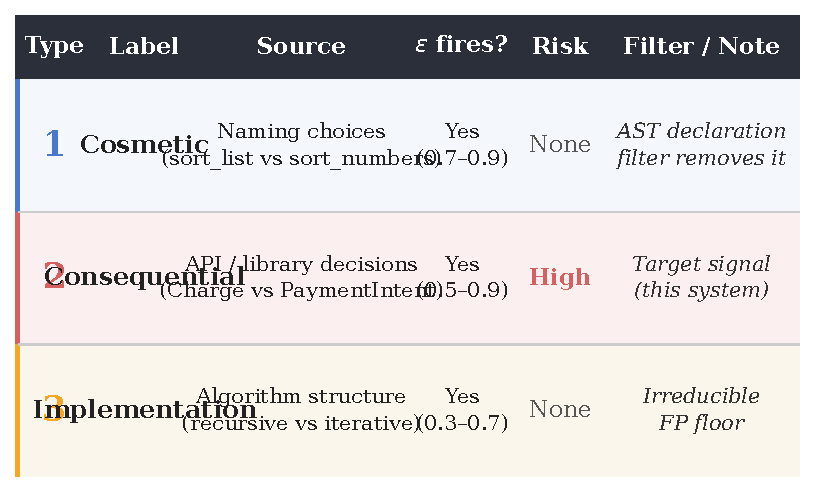
\includegraphics[width=0.85\textwidth]{figures/fig9_taxonomy.pdf}
\caption{The three-type uncertainty taxonomy. Type 1 is removed by AST
filtering; Type 3 is irreducible but rare in production API-integration
code; Type 2 is the signal the system is designed to catch.}
\label{fig:taxonomy}
\end{figure}

\subsection{AST filtering}
\label{subsec:ast}

We eliminate Type 1 via the generated code's AST. After stripping
markdown fences and parsing with Python's \texttt{ast}, we identify
\emph{declaration positions} --- source ranges where the model is
choosing a name rather than an API.
\textbf{Filtered:} function/method names, parameter names
(\texttt{ast.arg}), local variable names (\texttt{ast.Name} in
\texttt{Store}).
\textbf{Retained:} import targets, attribute accesses, keywords, type
annotations. Token-to-declaration matching uses range overlap (BPE
introduces a leading space); a pure-identifier guard prevents over-%
filtering of delimiter-prefixed tokens such as \texttt{(db}.

\begin{table}[h]
\centering
\small
\begin{tabular}{lc}
\toprule
\textbf{Configuration} & \textbf{LOW FP rate} \\
\midrule
Naive token entropy (no filtering)                & $90\%$ \\
+ Whitespace / comment filtering                   & $90\%$ \\
+ System prompt naming conventions                 & $60\%$ \\
+ AST declaration filtering                        & $60\%$ \\
+ Fence-format stripping                           & $50\%$ \\
\midrule
Residual (Type 3 only)                             & $50\%$ \\
\bottomrule
\end{tabular}
\caption{Successive filtering stages on 10 LOW prompts. Naming-%
convention prompt and AST filter are partially overlapping; without
the prompt, AST filtering alone drops FP from $90\%$ to $70\%$.
Residual $50\%$ is Type 3, rare in production API-integration code.}
\label{tab:filtering}
\end{table}

\subsection{Aggregation: max vs.\ mean}
\label{subsec:aggregation}

We aggregate with
$\eps_\text{file} = \max\{\eps_t : t \text{ retained}, \eps_t > \delta\}$,
$\delta = 0.30$. The compound alternative
$1 - \prod(1 - \eps_t)$ converges to $1.0$ for any non-trivial function.
Across all $90$ runs of the benchmark ($3 \times 30$), max and mean
produced identical fire/no-fire decisions at every threshold; we prefer
max because it localizes uncertainty to a specific actionable token.

\subsection{Thresholds and tiers}
\label{subsec:tiers}

Four tiers: \textsc{complete} ($\eps < 0.30$), \textsc{flagged}
($0.30 \le \eps < 0.65$), \textsc{paused} ($0.65 \le \eps < 0.95$),
\textsc{aborted} ($\eps \ge 0.95$). These are UX signals, not
calibrated probabilities --- empirical failure rates are $27\%/29\%/31\%$
(\S\ref{sec:evaluation}), monotonic but weakly ordinal. The load-%
bearing boundary is the binary \textsc{complete} vs.\ \textsc{flagged+}:
everything \textsc{flagged+} is forwarded to the stage-2 reviewer.

\subsection{Adaptive ensemble}
\label{subsec:ensemble}

The production implementation refines tier placement within
\textsc{flagged+} using a rolling mean-$\eps$ baseline and a top-$1$
logprob check; neither affects the binary \textsc{flagged+} gate.
Conformal calibration is left to future work.
